% !TEX root = diss.tex

\chapter{Do non-redox active metal cations have the potentials to behave as chemo-protective agents? The Effects on Metal Cations on HAT Reaction Barrier Heights}
\label{ch:hat}

\section{Introduction}

Metal cations are ubiquitous in biological systems and play an important role in biological function. As such, there is a great deal of interest in studying metals in biological systems. Proteins in particular are often associated with metals, and in the worldwide Protein Data Bank,\cite{Harding2010, Berman2007} over one-third of crystal structures contain metals. Redox active metals, such as copper and iron, act as co-factors in metalloenzymes for important catalytic processes.\cite{Atkins2010}

Non-redox active metal cations are equally as important in biological function as redox active metals, where they are essential to protein structure and function, along with cellular and neuronal signaling.\cite{Karp1999} Sodium and calcium ions are most abundant extracellurly, while potassium and magnesium are dominant inside of cells. While specific ionic concentrations vary dramatically dependening on physiological conditions, estimates for equilibrium concentrations in both mammalian heart cells\cite{Ingwall2006} and blood plasma\cite{daSilva2001} are listed in~\ref{tab:metalconc}. As sodium and magnesium are most abundant alkali and alkaline earth metals found in biologically relevant systems, they are of prime interest for investigation.

\begin{table}[!htbp]
  \caption{Ionic concentrations inside a mammalian heart cell and in the blood plasma. Concentrations are in units of mM. Values are rounded to one significant figure. Data are from Ref. \protect\citenum{Ingwall2006} and \protect\citenum{daSilva2001}.}
  \label{tab:metalconc}
\begin{tabular}{l c c}
  Ion Conc. & Mammalian Cells & Blood Plasma \\
  \hline
  \ch{Na^+} & 10 & 100--200 \\
  \ch{Mg^{2+}} & 10 & 1 \\
  \ch{K^+} & 100 & 4 \\
  \ch{Ca^{2+}} & 0.1 & 2
\end{tabular}
\end{table}

Extensive crystallographic surveys indicate that metals bind predominantly to oxygen centres in proteins.\cite{Harding1999, Harding2004, Hsin2008} Divalent metals are most often found bound directly to proteins. Calcium binds anywhere from 4 to 6 binding sites in protein crystal structures, while magnesium binds only 1 or 2. Monovalent metals, on the other hand, are often heavily solvated and so they appear in solvent cavities of proteins, although sodium or potassium are sometimes found bound directly to carbonyl or carboxylate oxygen centres.\cite{Harding2010}

A great deal of research has focussed on \ch{Ca^{2+}} in the context of reactive oxygen-centred radical production.\cite{Goerlach2015} Specifically, \ch{Ca^{2+}} ions are important in the mitochondria, where, depending on physiological conditions and concentrations, they can act as inhibitor or promoters of free-radical production in the electron transport chain.\cite{AdamVizi2010} In explanation is that \ch{Ca^{2+}} induce conformational changes of the proteins involved in the electron transport chain which are responsible for radical generation.\cite{Brookes2004} Mitochondrial free-radicals, when present in moderate amounts, can act as cell signalling molecules to activate pro-growth responses.\cite{Sullivan2014} However, ``dysfunctional'' mitochondria can produce excess radicals leading to oxidative damage which has been linked to degenerative diseases.

Given the significant importance alkali and alkaline earth metals play in biological systems, their impact on protein oxidation must be considered. However, until recently, kinetic studies of protein oxidation have not investigated the mechanistic role of non-redox active metals. In a series of three papers,\cite{Salamone2013a, Salamone2015metals, Salamone2016} Bietti and colleagues have shown that alkali and alkaline earth metals have an inhibitory effect on HAT reactions involving \cumo\ and organic substrates. Some of the experimental rate constants from these papers are summarized in~\ref{tab:hat-metals}. All rate constants were obtained by time-resolved LFP in nitrogen or argon-saturated acetonitrile (MeCN) at 298 K, as was previously described in Section~\ref{sec:hat-methods}. All of the experimental results have been rationalized on the basis of Lewis acid metals cations interactions with Lewis basic substrates.

\bgroup
\def\arraystretch{1.2}%  1 is the default, change whatever you need
\begin{table}
  \caption{Table summary of experimental data - Needs completion}
  \label{tab:hat-metals}
  \hspace*{-1.2cm}
  \begin{tabular}{l l c c}
    Substrate & Conditions & $k_H$ (\Ms) & $k_H$(MeCN)/$k_H$(M$^{n+}$) \\
    \hline
    1,4-cyclohexadiene &    & 6.7\E{7} & \\
    (CHD)  & \ch{LiClO4} 1.0 M & 7.5\E{7} & 0.89 \\
     & \ch{Mg(ClO4)2} 1.0 M & 7.0\E{7} & 0.96 \\
    tetrahydrofuran &   & 5.7\E{6} & \\
    (THF) & \ch{LiClO4} 1.0 M & 2.9\E{6} & 1.7 \\
     & \ch{LiOTf} 1.0 M & 2.8\E{6} & 2.0 \\
     & \ch{Mg(ClO4)2} 1.0 M & 1.8\E{6} & 3.2 \\
    triethylamine &  & 2.0\E{8} & \\
    (TEA) & \ch{LiClO4} 1.0 M & 9.4\E{7} & 2.1 \\
     & \ch{Mg(ClO4)2} 0.005 M & $<$1\E{6} & $>$200 \\
    $N,N$-dimethylformamide & & 1.2\E{6} & \\
    (DMF) & \ch{LiClO4} 0.5 M & $k_{H1}$ = 8.9\E{5} & 1.3 \\
      & & $k_{H2}$ = 1.5\E{6} & 0.80 \\
      & \ch{NaClO4} 0.2 M & $k_{H1}$ = 9.6\E{5} & 1.3 \\
      & & $k_{H2}$ = 1.4\E{6} & 0.86 \\
      & \ch{Mg(ClO4)2} 0.2 M & $k_{H1}$ = 5.8\E{5} & 2.1 \\
      & & $k_{H2}$ = 1.1\E{6} & 1.1 \\
      & \ch{Ca(ClO4)2} 0.2 M & $k_{H1}$ = 1.0\E{6} & 0.83 \\
    $N,N$-dimethylacetamide &  & 1.2\E{6} & \\
    (DMF) & \ch{LiClO4} 0.2 M & $k_{H1}$ = 8.5\E{5} & 1.4 \\
      & & $k_{H2}$ = 1.5\E{6} & 0.8 \\
      & \ch{NaClO4} 0.2 M & $k_{H1}$ = 1.1\E{6} & 1.1 \\
      & & $k_{H2}$ = 1.3\E{6} & 0.92 \\
      & \ch{Mg(ClO4)2} 0.2 M & $k_{H1}$ = 4.7\E{5} & 2.6 \\
      & & $k_{H2}$ = 2.4\E{5} & 5.0 \\
      & & $k_{H3}$ = 1.1\E{6} & 1.1 \\
      & \ch{Ca(ClO4)2} 0.2 M & $k_{H1}$ = 1.2\E{6} & 1.0
  \end{tabular}
\end{table}
\egroup

Firstly, for hydrocarbons, cyclic ethers, and tertiary amines, \cumo\ hydrogen abstraction rate constants in the presence of excess concentrations of lithium and magnesium salts were measured.\cite{Salamone2013a} In the presence of \ch{LiClO4} and \ch{Mg(ClO4)2}, the rate of abstraction by \cumo\ from 1,4-cyclohexadiene (CHD) increases very slightly. Since CHD has no Lewis basic centres, the increase in HAT rate constant was explained on the basis of metal cation interactions with \cumo, very slightly increasing the hydrogen abstraction ability by withdrawing electron density from the aromatic ring. Metal cations were also shown to increase the unimolecular decay of \cumo\ by $\beta$-scission (See Section~\ref{sec:hat-methods}). The largest kinetic effect was observed with \ch{LiClO4} with $k_\beta$ = 1.8\E{6} $s^{-1}$, which is a
roughly 3-fold increase as compared to the rate in MeCN at 298 K ($k_\beta$\cite{Avila1995} = 6.3\E{5} $s^{-1}$). This effect is significantly less than the observed kinetic solvent effect on \cumo\ $\beta$-scission measured in \ch{H2O} or 2,2,2-trifluoroethanol ($k_\beta$ = 1.0\E{7} and 6.1\E{6} $s^{-1}$, respectively).\cite{Bietti2005, Neta1984} Therefore, the kinetic effects of these alkali and alkaline metal salts interacting via Lewis acid-base interactions with the oxygen-centre of \cumo\ are less than the effects of hydrogen-bonding by solvents.

Next, the HAT rate constants for abstraction from tetrahydrofuran (THF) decrease in the presence of non-redox active metal salts. Both \ch{LiClO4} and \ch{LiOTf} decrease $k_H$ by a factor of about 2, indicating the nature of the counter-anion plays a negligible role in the Lewis acid-base interactions between metal cations and substrates. The addition of \ch{Mg(ClO4)2} has a greater effect on HAT reactivity, decreasing $k_H$ by a factor of 3. Magnesium ions are a stronger Lewis acid than lithium,\cite{Fukuzumi2002} supporting the notion of Lewis acid-base interactions between the oxygen lone-pair and the metal cations. The decrease in $k_H$ has been partially attributed to the reduction in hyperconjugative overlap between the oxygen lone-pair and the neighbouring \ch{C-H} $\sigma^*$ anti-bonding orbital (See~\ref{fig:THF}), as a consequence of the metal cation withdrawing electron density from the oxygen lone-pair.

A 2-fold decrease in $k_H$ for the tertiary amine, triethylamine (TEA), is observed upon the addition of \ch{LiClO4}, for which an analogous orbital interaction explanation is also appropriate. Interestingly, the addition of 1.0 M \ch{Mg(ClO4)2} was reported to immediately form a precipitate to form. This precipitate was identified as the formation of a strong TEA-\ch{Mg^{2+}} Lewis acid-base adduct. This observation is once again consistent with the stronger Lewis acidity of \ch{Mg^{2+}} as compared to \ch{Li^+}, and also the significantly greater Lewis basicity of TEA vs THF.\cite{Salamone2013a, Reichardt2010} It was also pointed out that MeCN will competitively bind with metal cations, however it is a weaker Lewis base than both THF and TEA. Measurements of $k_H$ for HAT between \cumo\ and TEA in the presence of 0.005 M \ch{Mg(ClO4)2} were successful only up until [TEA] = 9.6 mM, at which point a precipitate began to form. Nonetheless, an upper limit to the hydrogen abstraction rate constant was estimated as $k_H <$ 1\E{6} \Ms, or at least a 200 fold decrease relative to no metal salt. Very similar results for bulkier tertiary amines were also obtained. Thus, the presence of strong Lewis acids in the presence of Lewis basic sites on hydrogen atom donors can deactivate \ch{C-H} bonds.

Next, we turn to the more relevant models for the work of this thesis, the tertiary amides $N,N$-dimethylformamide (DMF) and $N,N$-dimethylacetamide (DMA). As with THF, normal hyperconjugative overlap between the conjugated amide $\pi$-system and the adjacent \ch{C-H} $\sigma^*$ anti-bonding orbitals weakens the C-H bonds. Therefore, metal binding to the amide oxygen-centre should result in a decrease in this orbital interaction, strengthen the C-H bonds, and decrease HAT reactivity. In their study, \citet{Salamone2015metals} measured \cumo\ abstraction rate constants from DMF and DMA in the presence of stoichiometric equivalents of \ch{LiClO4}, \ch{LiOTf}, \ch{NaClO4}, \ch{Mg(ClO4)2}, and \ch{Ca(ClO4)2} (in contrast to the excess used in Reference~\citenum{Salamone2013a}). Figure~\ref{fig:k-metals-mg}a,b shows the plots of $k_{obs}$ against [substrate] for the reactions of \cumo with DMF and DMA in MeCN containing 0.2 M \ch{Mg(ClO4)2}, respectively. For both DMF and DMA, there are three distinct regions in the plots: weak C-H bond activation for [amide]/[\ch{Mg^{2+}}]$\leq 2$, followed by strong C-H bond deactivation for 2$<$[amide]/[\ch{Mg^{2+}}]$\leq$4, and no deactivation for [amide]/[\ch{Mg^{2+}}]$<$4.

\begin{figure}[!htbp]
  \includegraphics[width=\textwidth]{figures/kH-dma-dmf-mgclo42.png}
  \caption[Plot of observed rate constant against concentration of DMF and DMA for reaction with \cumo\ at 298 K in the presence of 0.2 M \ch{Mg(ClO4)2}.]
  {\textbf{a)} Plot of observed rate constant against concentration of DMF for reaction with \cumo\ at 298 K in the presence of 0.2 M \ch{Mg(ClO4)2}. 0--0.4 M [DMF] range (black circles), $k_{H1}$ = 5.8\E{5} \Ms; 0.8--2.2 M [DMF] range (white circles), $k_{H2}$ = 1.3\E{6} \Ms.
  \textbf{b)} Plot of observed rate constant against concentration of DMA for reaction with \cumo\ at 298 K in the presence of 0.2 M \ch{Mg(ClO4)2}. 0--0.4 M [DMA] range (black circles), $k_{H1}$ = 4.7\E{5} \Ms; 0.4--0.8 M [DMA] range (grey circles), $k_{H2}$ = 2.4\E{5} \Ms; 0.8--2.2 M [DMA] range (white circles), $k_{H3}$ = 1.1\E{6} \Ms. Reprinted with permission from Reference~\protect\citenum{Salamone2015metals}. Copyright 2015 American Chemical Society.}
  \label{fig:k-metals-mg}
\end{figure}

The addition of both \ch{LiClO4} and \ch{LiOTf} decrease to a similar extent the rate constants for abstraction from DMF and DMA by \cumo. However, in contrast to \ch{Mg(ClO4)2}, the lithium salts strongly deactivate \ch{C-H} bonds for 2 equivalents, followed by weak deactivation for another 2 equivalents, and no deactivation for [amide]/[\ch{Li^{+}}]$<$4. Salamone et al. were not able to give a clear cut explanation, but suggest that the different patterns are a result of differences in charge density, which is greater for \ch{Mg^{2+}} than \ch{Li^+}, as well as different coordination geometries of the two ions. A coordination number of 4 is most common for \ch{Li^+}, while an octahedral geometry with the coordination of 6 ligands is almost always observed for \ch{Mg^{2+}}.\cite{Babu2013, Dudev2014} As a result, interactions of the ions with solvent and counter-anions are suggested to be more important for \ch{Mg^{2+}} than \ch{Li^+}.

\ch{NaClO4} and \ch{Ca(ClO4)2} influence HAT between \cumo\ and DMA to different extents than both \ch{LiClO4} and \ch{Mg(ClO4)2}. Figure~\ref{fig:k-metals-naca}a,b shows the plots of $k_{obs}$ against [substrate] for the reactions of \cumo with DMA in MeCN containing 0.2 M \ch{NaClO4} and \ch{Mg(ClO4)2}, respectively. For \ch{NaClO4}, an almost negligible deactivation of \ch{C-H} bonds is observed for up to 4 equivalents of DMA. This was explained on the basis of the weaker Lewis acidity of \ch{Na^+} as compared to \ch{Li^+}. With regards to \ch{Ca(ClO4)2}, binding to DMA fully deactivates \ch{C-H} bond abstraction up to 4 equivalents of DMA. The first region of~\ref{fig:k-metals-naca}b ([DMA] = 0--0.2 M, black circles) represents the decrease in $k_\beta$ of \cumo as \ch{Ca^{2+}} preferentially binds to DMA over \cumo. These results show that Lewis acid-base interactions between alkali or alkaline earth metal cations can greatly depress hydrogen abstraction by alkyoxyl radicals.

\begin{figure}[!htbp]
  \includegraphics[width=\textwidth]{figures/exptdma-na-ca.png}
  \caption[Plot of observed rate constant against concentration of DMA for reaction with \cumo\ at 298 K in the presence of 0.2 M \ch{NaClO4} and \ch{Mg(ClO4)2}.]
  {\textbf{a)} Plot of observed rate constant against concentration of DMA for reaction with \cumo\ at 298 K in the presence of 0.2 M \ch{NaClO4}. 0--0.8 M [DMA] range (black circles), $k_{H1}$ = 9.6\E{5} \Ms; 0.8--1.4 M [DMA] range (white circles), $k_{H2}$ = 1.4\E{6} \Ms.
  \textbf{b)} Plot of observed rate constant against concentration of DMA for reaction with \cumo\ at 298 K in the presence of 0.2 M \ch{Ca(ClO4)2}. 0.8--1.7 M [DMA] range (white circles), $k_{H1}$ = 1.2\E{6} \Ms. Adapted with permission from Reference~\protect\citenum{Salamone2015metals}. Copyright 2015 American Chemical Society.}
  \label{fig:k-metals-naca}
\end{figure}

Finally, \citet{Salamone2016} examined the effects of substrate structure on HAT reaction between \cumo and tertiary alkanamides in the presence of alkali and alkaline earth metal ions. For $N,N$-dialkylacetamides, the steric bulk of the $N$-alkyl groups was previously characterized.\cite{Salamone2014} Steric repulsion between \cumo\ and the $N$-alkyl groups can decreases the HAT rate constant, as evident by the 3-fold decrease in $k_H$ in going from DMA to $N,N$-diisobutylacetamide (DIA; 1.2\E{6} and 3.1\E{5} \Ms, respectively). For reactions of \cumo\ with DIA addition of 0.2 M \ch{LiClO4} or \ch{Ca(ClO4)2} to results in the same trends in \ch{C-H} bond deactivation observed for DMA. This indicates that the influence of metal cation-substrate binding is not significantly influences by the steric bulk of $N$-alkyl groups.  The same is true for the addition of 0.2 M \ch{Mg(ClO4)2} to abstraction from DIA by \cumo, as shown in~\ref{fig:k-dia-mg}. Once again, an slight decrease in reactivity is observed for the first 2 equivalents of DIA, followed by strong C-H bond deactivation for an additional two equivalents, and no deactivation beyond that. No additional insight was provided by Salamone et al. as to the reason for this reactivity. The plausible explanation hypothesized was once again that \ch{Mg^{2+}} has a high charge density.

\begin{figure}[!htbp]
  \includegraphics[width=0.6\textwidth]{figures/exptdia-mg.png}
  \caption[Plot of observed rate constant against concentration of DIA for reaction with \cumo\ at 298 K in the presence of 0.2 M \ch{Mg(ClO4)2}.]
  {Plot of observed rate constant against concentration of DIA for reaction with \cumo\ at 298 K in the presence of 0.2 M \ch{Mg(ClO4)2}. 0--0.4 M [DIA] range, $k_{H1}$ = 3.6\E{5} \Ms; 0.8--1.4 M [DIA] range, $k_{H2}$ = 2.9\E{5} \Ms.
  Reprinted from Tetrahedron, 72, Salamone et al., Hydrogen atom transfer from tertiary alkanamides to the cumyloxyl radical. The role of substrate structure on alkali and alkaline earth metal ion induced \ch{C–H} bond deactivation, 7757--7763, 2016, with permission from Elsevier.}
  \label{fig:k-dia-mg}
\end{figure}

With these results in mind, I am interested in the possibility that alkali and alkaline earth metal cations found in biological system can protect \ch{C-H} bonds in proteins from HAT to reactive oxygen-centred radicals. However, the experimental results do not answer some of the key physico-chemical determinants which may make this possible. Specifically, I have composed several important research questions which remain unclear from the experimental results.

The first question which I have is one of methodology: Can DFT-based methods can accurately treat alkali/alkaline metal cation binding to organic substrates or radicals? There exists limited ab initio data describing these interactions.\cite{ Siu2001, Corral2003, Suarez2011, Baldauf2013} Therefore, I have conducted a benchmark quality study involving \ch{Li^+}, \ch{Na^+}, \ch{Mg^{2+}}, \ch{K^+}, and \ch{Ca^{2+}}. to the best of my knowledge, this represents the first systematic benchmark study of these metal cations with both organic substrates, and radicals.

Secondly, the nature of the binding of metal ions to substrates is still poorly described, especially given the odd stoichiometric effects observed for \ch{Mg(ClO4)2} with alkanamides. Specifically, I wish to address the range of these interactions, and how much the metals do effect the C-H being broken. Throughout this investigation I have utilized both \ch{Na^+} and \ch{Mg^{2+}} in my calculations. These metal ions were chosen to capture the large differences in Lewis acidity and ion size associated with these third-period ions, and because they are two of the most biologically relevant metal ions.

Thirdly, I address the effect that metal ions have on the HAT barrier heights. Experiments demonstrate that under certain conditions the presence of metal ions can decrease HAT reactivity. If metal ions do effectively increase C-H bond strengths, this will certainly be a contributing factor to the free energy barrier. There will likely be additional factors such as polarization in the TS complex, or other effects of possible charge transfer from the substrate to metal ions. To investigate this, I have primarily studied HAT reactions involving DMA and oxygen-centred radicals.

\jnote{finish your thoughts here}

\section{Computational methods and details}

All quantum mechanical calculations were performed using either the Gaussian 09 software package,\cite{Frisch2009} or the TURBOMOLE software package.\cite{turbomole} Calculations for the benchmark quality data of metal binding to substrates were first optimized at the LC-$\omega$PBE-D3(BJ)/6-31+G(2d,2p) level of theory, and later re-optimized with larger 6-311+G(3df,3pd) basis sets. Single-point energy calculations were then carried out using the CCSD(T) methodology and various basis sets, as will be described in Section~\ref{sec:benchmark}. Final benchmark quality binding energies have been calculated using the F12$^*$ explicitly correlated method with Def2-QZVPPD primary basis sets and Def2-QZVPP auxiliary basis sets required for the resolution-of-the-identity (RI) approximation as implemented in TURBOMOLE. The RI approximation is used to reduce the computational cost associated with calculating MO integrals.\cite{note-book} At total of 31 different DFT-based methods with nearly complete 6-311+G(3df,3pd) and moderate 6-31+G(2d,2p) basis sets were tested both by single-point energy calculations on the benchmark structures. Geometry optimization calculations starting from the benchmark structures were also performed for three of the best performing DFT-based method, in order to verify their ability to capture the minimum energy bound structures.

To test the effects of metal cations on HAT barrier heights, calculations were first performed for the reactions not involving metal cations. Geometry optimizations were performed at the M05-2X/6-31+G$^{**}$ level of theory. Transition state (TS) structures were obtained by first freezing the abstraction donor-hydrogen-acceptor bond lengths with multiple initial orientations. The frozen bonds were then relaxed to obtain the final TS structures, which were then used to identify the appropriate pre- and post-reaction complexes. All structures were subjected to harmonic vibrational frequency calculations, which were visualized using the Chemcraft program\cite{ccraft} to verify minima (or saddle-points with a single imaginary frequency connecting reactants to products for TS structures). Single-point energy calculations were performed at the M05-2X/6-311+G(2d,2p) level of theory. The effects of MeCN solvent were estimated by inclusion of the SMD continuum solvent model in single-point energy calculations.


\section{Benchmarking DFT based methods for the binding of alkali and alkaline earth metals to organic substrates and oxygen centred radicals}
\sectionmark{Benchmarking DFT based methods}
\label{sec:benchmark}

The purpose of this work is to provide high-level binding energies for organic substrates which are of interest directly for this project, but also which may be useful for future work. The substrates proposed were to be relevant to simple biological models such as dipeptide like molecules and the hydroxyl and hydroperoxyl radical. We also wanted to incorporate substrates with are important to the physical organic experiments that are performed to probe these systems, thus solvents such as acetonitrile and dimethyl sulfoxide and the benzyloxyl and cumyloxyl radicals were also included. This set is shown in \ref{fig:set1}\jnote{FIND CDX}.

\begin{scheme}[hbt]
  \centering
    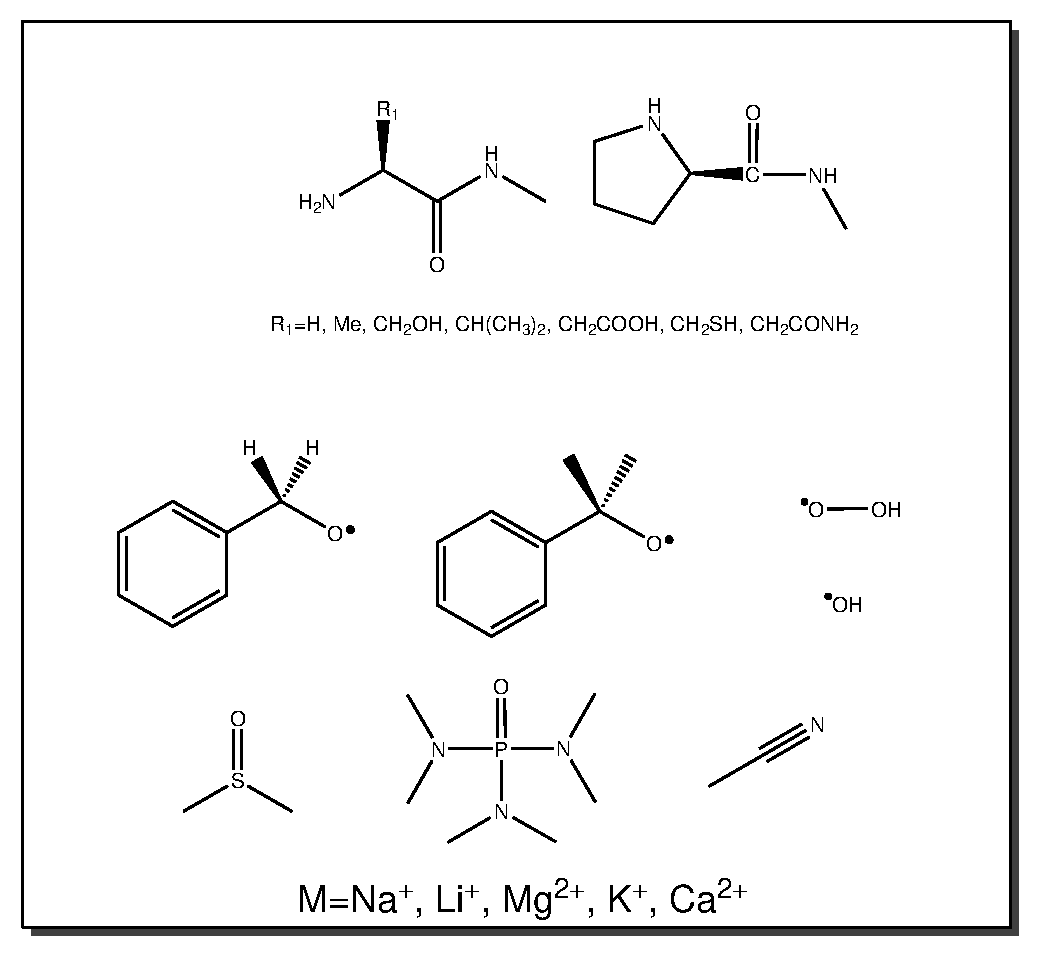
\includegraphics{figures/set1}
    \caption{Initial proposed benchmark set of molecules and cations. Note this set consistes of all combinations of substrates and metal cation, thus there are 60 complexes in the set.}
  \label{fig:set1}
\end{scheme}

Benchmark quality binding energies are generally calculated using the ``gold standard'' approach, CCSD(T)/CBS, where correlation consistent basis sets\jnote{(CITATION)} (cc-pV\emph{X}Z, \emph{X}=T,Q,5) developed by Dunning and co-workers are used for complete basis set extrapolation. These basis sets have limited availability for the metals of interest. Specifically, basis sets for K are note available, and only non-augmented basis sets for Li, Na, Mg, and Ca. It is necessary to include core correlation of the n-1 shell in alkali and alkaline earth metals, thus it is advantageous to use core valence basis sets such as cc-pCV\emph{X}Z. These basis sets are even more limitted, thus we opted for the augmented version of the polarization consistent basis sets of Jensen and co-workers (aug-pc-\emph{N}, \emph{N}=2,3,4). \jnote{CITATIONS FOR GOLD STANDARD AND BASIS SETS, NEED THEORY SECTION ON DIFFERENT BASIS SETS}

While performing CCSD(T)/CBS calculations, we notices that the metal cations (and neutral metal atoms), did not converge smoothly to the complete basis set limit. Given this, and the limited computational resources, we decided to re-evaluate the size scope of the benchmark set being used. In order to facilitate future DFT work and probe the issue of basis set convergence of alkali and alkaline earth metals, a benchmark set of small substrates was proposed. This new set is shown in \ref{fig:set2}. The new, small benchmark set was selected to include important functional groups and radicals for biological systems and the most common solvent used in physical organic experiments, acetonitrile.

\begin{scheme}[!htbp]
  \centering
    \includegraphics[width=\textwidth]{figures/set2.eps}
    \caption{Revised benchmark set of small substrates and cations. Note this set consists of all combinations of substrates and metal cations, i.e., there are 35 complexes in the set.}
  \label{fig:set2}
\end{scheme}

\subsection{Metal cation basis set convergence}

\subsection{High level results and evaluation of various density-functional theory methods}

\begin{table}[!htbp]
  \caption[Benchmark gas-phase binding energies of alkali and alkaline earth-metals with small organic substrates and radicals.]{Benchmark gas-phase binding energies of alkali and alkaline earth-metals with small organic substrates and radicals. Values are calculated at the CCSD(T)-F12$^*$/Def2-QZVPPD//LC-$\omega$PBE-D3(BJ)/6-311+G(3df,3pd) level of theory. All values are in \kcalmol.}\label{tab:ccsd-metal}
  \begin{tabular}{l c c c c c}
            &\ch{Li^+}&\ch{Na^+}&\ch{Mg^{2+}}&\ch{K^+}&\ch{Ca^{2+}}\\
    \hline
    \ch{H2O}    & -34.7 &  -24.4 &  -82.0  &  -17.8 &  -56.8 \\
    \ch{NH3}    & -39.9 &  -28.2 &  -98.1  &  -19.8 &  -65.3 \\
    MeCN        & -44.4 &  -33.0 &  -113.1 &  -24.9 &  -80.7 \\
    Formamide   & -50.7 &  -36.9 &  -128.2 &  -28.5 &  -96.1 \\
    Formic acid & -38.4 &  -27.0 &  -101.9 &  -20.0 &  -72.6 \\
    \ch{HO^.}   & -21.3 &  -16.8 &  -57.0  &  -12.4 &  -40.7 \\
    \ch{HOO^.}  & -27.1 &  -19.1 &  -72.2  &  -13.9 &  -49.0
  \end{tabular}
\end{table}


\begin{longtable}[!htbp]{m{3.1cm} c c | c c}
\caption[Evaluation of DFT-based methods for alkali and alkaline metal binding to organic substrates and radicals.]{Evaluation of DFT-based methods for alkali and alkaline metal binding to organic substrates and radicals. All values are in \kcalmol. Negative values indicate underbinding.}
\label{tab:dft-metal}\\
\textbf{Method}&\textbf{MAE}&\textbf{Max./Min}&\textbf{MAE}&\textbf{Max./Min.}\\
\hline
 & \multicolumn{2}{c|}{6-311+G(3df,3pd)} & \multicolumn{2}{c}{6-31+G(2d,2p)}\\
B3LYP             &  1.49 &  5.12/-0.57  &  1.59 &  4.67/-7.28 \\
B3P86             &  0.94 &  3.87/-0.96  &  1.36 &  1.99/-7.38 \\
B3PW91            &  0.95 &  2.74/-1.64  &  1.89 &  1.47/-8.76 \\
BH+HLYP           &  1.89 &  5.29/-0.59  &  1.93 &  4.65/-5.64 \\
BLYP              &  1.60 &  5.56/-1.51  &  1.88 &  5.30/-8.80 \\
BMK               &  0.90 &  1.13/-2.40  &  1.98 &  0.86/-8.75 \\
BP86              &  1.63 &  4.61/-3.21  &  2.27 &  1.55/-9.38 \\
CAM-B3LYP         &  2.40 &  6.25/ 0.21  &  1.98 &  5.82/-5.25 \\
LC-$\omega$PBE    &  0.78 &  2.95/-0.73  &  1.34 &  2.19/-8.00 \\
M05-2X            &  1.11 &  3.21/ 0.15  &  1.24 &  2.55/-5.75 \\
M06               &  1.05 &  2.36/-4.83  &  1.83 &  1.76/-9.03 \\
M06-2X            &  1.13 &  3.68/ 0.11  &  1.26 &  3.00/-6.63 \\
M06L              &  1.52 &  2.64/-6.94  &  2.55 &  1.21/-11.2 \\
MOHLYP            &  2.30 &  1.52/-5.40  &  4.04 &  0.89/-15.2 \\
PBE0              &  1.22 &  4.19/-0.31  &  1.25 &  3.30/-7.25 \\
PBE               &  1.70 &  6.09/-0.87  &  1.58 &  4.68/-8.15 \\
TPSS              &  1.38 &  4.88/-1.12  &  1.60 &  2.91/-8.12 \\
B97D3             &  1.50 &  5.94/-2.19  &  1.69 &  2.67/-8.41 \\
$\omega$B97       &  0.61 &  2.13/-1.72  &  1.41 &  1.78/-7.57 \\
$\omega$B97XD     &  1.12 &  1.02/-4.52  &  2.24 &  0.65/-8.64 \\
HSEH1PBE          &  1.30 &  4.28/-0.16  &  1.23 &  3.45/-6.95 \\
B3LYP-D3(BJ)      &  2.86 &  7.50/ 0.34  &  1.92 &  7.05/-4.33 \\
BLYP-D3(BJ)       &  2.89 &  8.40/-0.14  &  1.83 &  8.14/-5.30 \\
B3PW91-D3(BJ)     &  1.47 &  5.81/-0.44  &  1.02 &  3.88/-5.69 \\
BMK-D3(BJ)        &  1.03 &  4.05/-1.06  &  1.02 &  2.03/-5.49 \\
BP86-D3(BJ)       &  1.77 &  7.78/-1.05  &  1.26 &  3.96/-6.19 \\
CAM-B3LYP-D3(BJ)  &  3.19 &  7.50/ 0.78  &  2.27 &  7.07/-3.54 \\
LC-$\omega$PDE-D3(BJ)& 1.47 & 4.07/-0.06 &  1.33 &  3.30/-6.15 \\
PBE0-D3(BJ)       &  1.92 &  5.37/ 0.20  &  1.33 &  4.47/-5.74 \\
PBE-D3(BJ)        &  2.24 &  7.57/-0.22  &  1.44 &  5.90/-6.67 \\
TPSS-D3(BJ)       &  2.03 &  6.93/-0.30  &  1.25 &  4.56/-6.03
\end{longtable}

\begin{table}
  \caption[Comparison of single point and relaxed binding energies for alkali and alkaline metal binding with DFT-based methods.]{Comparison of single point (SP on benchmark structure) and relaxed (optimized with method) binding energies for alkali and alkaline metal binding with DFT-based methods and 6-31+G(2d,2p) basis sets. Mean absolute error (MAE) values are in \kcalmol and average root mean squared deviation of geometry are in \AA.}\label{tab:ccsd-metal-opt}
  \begin{tabular}{l c c c}
    Method & MAE(SP) & MAE(Relaxed) & Average(RMSD) \\
    \hline
    BMK-D3(BJ) & 1.02 & 1.24 & 0.012 \\
    M05-2X & 1.24 & 1.17 & 0.020 \\
    TPSS-D3(BJ) & 1.25 & 1.21 & 0.026 \\
  \end{tabular}
\end{table}

\section{Exploring the nature of metal cation substrate interactions}

\begin{figure}[!htbp]
\centering
\vspace{1.0cm}
\hspace*{-1.8cm}
\begin{minipage}{8cm}
  \centering
  \begin{overpic}[width=\textwidth]{figures/pes_dma_na}
  \put(5,70) {\large\textbf{A.}}
\end{overpic}
\end{minipage}%
\begin{minipage}{8cm}
  \centering
  \begin{overpic}[width=\textwidth]{figures/pes_dma_nacl}
  \put(5,70) {\large\textbf{B.}}
\end{overpic}
\end{minipage}
\caption[Potential energy surface of binding energy between DMA and sodium cation and sodium chloride.]{Potential energy surface of binding energy between DMA and \textbf{A} sodium cation and \textbf{B} sodium chloride as a function of O-Na interaction distance (\AA). Black line and points is gas-phase, grey squares and line is in continuum MeCN solvent, and white circles and dashed line is in continuum water solvent. Calculated as a rigid scan from the M05-2X/6-31+G$^{**}$ minimized structure at the M05-2X/6-311+G(2d,2p) level of theory with the SMD solvent model.}
\label{fig:pes-dma-na}
\end{figure}

\begin{figure}[!htbp]
\centering
\vspace{1.0cm}
\hspace*{-1.8cm}
\begin{minipage}{8cm}
  \centering
  \begin{overpic}[width=\textwidth]{figures/pes_dma_mg}
  \put(5,70) {\large\textbf{A.}}
\end{overpic}
\end{minipage}%
\begin{minipage}{8cm}
  \centering
  \begin{overpic}[width=\textwidth]{figures/pes_dma_mgcl2}
  \put(5,70) {\large\textbf{B.}}
\end{overpic}
\end{minipage}
\caption[Potential energy surface of binding energy between DMA and magnesium cation and magnesium chloride.]{Potential energy surface of binding energy between DMA and \textbf{A} magnesium cation and \textbf{B} magnesium chloride as a function of O-Mg interaction distance (\AA). Black line and points is gas-phase, grey squares and line is in continuum MeCN solvent, and white circles and dashed line is in continuum water solvent. Calculated as a rigid scan from the M05-2X/6-31+G$^{**}$ minimized structure at the M05-2X/6-311+G(2d,2p) level of theory with the SMD solvent model.}
\label{fig:pes-dma-mg}
\end{figure}
